\documentclass[12pt,letterpaper]{report}

\usepackage[spanish]{babel}
\usepackage[utf8]{inputenc}
\usepackage[right=2cm,left=3cm,top=2cm,bottom=2cm,headsep=0cm,footskip=0.5cm]{geometry}
\usepackage{graphicx}
\usepackage{float}
\usepackage{wrapfig}
\usepackage{amsmath, amsthm, amssymb, amsfonts}

\newtheorem*{definition}

\frenchspacing
\title{\Huge Diccionarios \\ Tarea 3 - Diseño y Análisis de Algoritmos \\ Informe}
\author{Nicolás Salas V.}
\def\thesection       {\arabic{section}}
\sloppy

\begin{document}
\begin{figure}[t]

\includegraphics[scale=0.83]{logo.png}
%\hspace{3.5cm}
\begin{tabular}{l}
\small Universidad de Chile\\
\small Facultad de Ciencias Físicas y Matemáticas\\
\small Departamento de Ciencias de la Computación\\
\small CC4102 Diseño y Análisis de Algoritmos\\
\small Prof: Gonzalo Navarro B.
\vspace{2.3cm}
\end{tabular}
\end{figure}

\maketitle

\tableofcontents
\newpage

\section{Introducción}
El objetivo de este informe es comparar las implementaciones de diccionarios mediante \'arboles de b\'usqueda. En particular se estudiar\'a los siguientes casos:

\begin{itemize}
\item \'Arbol de b\'usqueda binaria
\item \'Arbol AVL
\item Splay Tree
\end{itemize}

Interesa -como en cualquier experimento de eficiencia de estructuras- saber cu\'al es la mejor estructura posible para implementar diccionarios. De nuevo, el experimento es entre las cuatro estructuras antes mencionadas. Hay otras estructuras que implementan diccionarios que pueden ser mejores, pero se quiere evaluar estas tres.\\

Aunque lo ideal sería encontrar una estructura que fuese mejor que todas las otras, esto probablemente no ocurrirá\footnote{Sobre esto se discute en la próxima sección, de Hipótesis.}, debido a las implementaciones de cada estructura. Con esa limitante, interesa saber cuáles son las mejores estructuras para qué casos.\\

Para partir, se expone un pequeño resumen de cada estructura de datos, que se analizarán a fondo en la sección de Marco Teórico. Se asumen conocimientos básicos de computación, en particular se asume que se conoce lo que es una estructura de datos, lo que significa recursividad y dominio básico de punteros. En los anexos se muestra dónde se puede investigar lo que son estos conceptos.\\

\subsection{Árbol de Búsqueda Binaria}
\label{subsec:expl_abb}

Un Árbol de Búsqueda Binaria no es más que una estructura de datos que almacena un dato comparable y dos punteros a hijos que también son árboles. Este árbol cumple con la propiedad de que todos los elementos almacenados en los nodos de su subárbol izquierdo son menores al valor almacenado en el nodo \emph{raíz} y de igual manera, los elementos almacenados en los nodos de su subárbol derecho con mayores al valor de la raíz. \textbf{Esta propiedad la cumple tanto este tipo de árbol como los árboles AVL, los Splay Trees y otro tipo de árboles que no se estudian en este experimento}. La inserción y borrado se explica en la sección de diseño experimental, pero es importante tener en cuenta que dichas operaciones \textbf{no rearreglan el árbol}, de manera que la búsqueda no siempre cumple con la propiedad de ser logarítmica.

\subsection{Árbol AVL}
\label{subsec:expl_avl}
Un Árbol AVL es un árbol de búsqueda binaria, pero que rearregla sus elementos a medida que se insertan, para mantenerse balanceado, en inglés este tipo de estructuras se llaman \emph{self balancing binary search tree}, que significa Árbol de Búsqueda Binaria Autobalanceado. Los AVL mantienen la diferencia de altura de sus dos subárboles constante, con ello se asegura que el tiempo de búsqueda, y en general de las operaciones sobre estos árboles sea logarítmica.

\subsection{Splay Tree}
\label{subsec:expl_splay}

Un Splay Tree es un árbol de búsqueda binaria que no se preocupa de mantenerse balanceado\footnote{En cierto modo, sí lo hace, pero esta perspectiva se abordará en el Marco Teórico.}, sino que su preocupación principal es mantener los elementos accesados con mayor frecuencia \emph{más arriba} en el árbol. Es decir, minimiza el número de comparaciones (o, dicho de otra manera, accesos a nodos) para elementos que son buscados frecuentemente.

\subsection{Mediciones}
\label{subsec:mediciones}

Para comparar la efectividad de cada una de estas estructuras de datos, es necesario tomar algunos parámetros objetivos. En este caso, un buen parámetro que nunca falla es \textbf{el tiempo}. Además, es conocido que algunas estructuras pesan más que otras, así que también se medirá el \textbf{Tamaño ocupado por cada estructura}. En base a estas dos mediciones se pueden inferir otras medidas de rendimiento, o incluso comparar los resultados reales contra la teoría. Esto se expone en las secciones de Resultados y Análisis de Datos.

\newpage
\section{Hipótesis}
Ya conociendo a grandes rasgos lo que hace cada árbol es posible elaborar algunas hipótesis sobre este experimento, y por supuesto, los argumentos para que ello sea así.\\

Los Splay Tree no se quedan en la noción de que todo árbol debe ser balanceado. ?`Por qué deberían balancearse elementos que nunca van a ser buscados en una estructura? Esta simple noción hace que sean una estructura mucho más adaptada a la realidad, donde la cantidad de elementos que se buscan está -haciendo una estimación generosa- no más allá del 20\% de los elementos\footnote{En verdad, esta afirmación sobre los splay trees adaptándose a la realidad tiene que ver con la predilección del autor por esta estructura. De todas maneras, lo expuesto no dista mucho de la realidad}. O sea, los Splay Trees han de ser mucho mejores que los otros tipos de árboles para casos reales, justamente porque lo que más se busca siempre está ``a mano''.\\

Sobre los Árboles de Búsqueda Binaria (en adelante \emph{ABB}) y AVL es sabido que los ABB tienen casos degenerados en los que se comportan como si fuesen listas enlazadas, esto pasa específicamente cuando los elementos se insertan ordenadamente. Este es un caso más bien extraño, pero en ningún momento imposible, de manera que los AVL son mejores que los ABB para casos degenerados. Sin embargo, en la teoría los AVL son mejores que los ABB, porque sus costos son siempre $O(\log n)$, pero lo que la notación obvía, es que existe un costo adicional -en la literatura es conocido como \emph{overhead}- asociado a el rebalanceo en la inserción y borrado. Los experimentos deberían indicar que, en promedio, los AVL se demoran más en insertar y borrar que los ABB.\\

Sobre el espacio, el árbol AVL ocupa $O(1)$ espacio más que un ABB convencional por nodo, puesto que cada uno debe almacenar su altura para poder rebalancearse, esto hace que los AVL sean más pesados que los ABB. Por otro lado, los Splay Tree no tienen overhead asociado al espacio, puesto que el reordenamiento de nodos no implica necesariamente rebalanceo, así que para espacio los Splay Tree deberían tener siempre el mismo espacio que los ABB.\\

La discusión anterior puede dar una última hipótesis sobre los Splay Tree comparados con los ABB. Entre ellos dos no hay diferencias de espacio, y respecto de los costos de las operaciones, ABB tiene costo \textbf{promedio} $O(n)$, mientras que los Splay Tree tienen costo \textbf{amortizado} $O(n)$. Vale la pena discutir cuál es mejor usar en la práctica, porque ambos costos son conceptualmente muy parecidos, y ambos ocupan el mismo espacio para la estructura de datos. Para conjeturar, los Splay Tree debieran ser mejores que los ABB \textbf{si es que no se sabe nada del input}, pero los ABB deberían ser mejor si se tiene la certeza de que el input viene desordenado.\\

Resumiendo:

\begin{enumerate}
\item Un Splay Tree se comporta mejor si hay elementos con mayores probabilidades de acceso que otros.
\item Un AVL es mejor en casos degenerados con probabilidades uniformes (o desconocidas) de acceso.
\item El mejor espacio está entre ABB y Splay Tree.
\item Los AVL ocupan más espacio que los Splay Tree y los ABB.
\end{enumerate}

\newpage
\section{Marco Teórico}
\label{sec:marco}

En esta sección el objetivo es explicar las estructuras de datos y sus algoritmos, de manera de poder entender mejor las hipótesis, resolver las dudas que puedan haber quedado en la introducción y tener la base para poder entender el diseño experimental que se ha hecho para esta experiencia.\\

En este experimento la implementación de diccionarios se ha hecho exclusivamente con árboles, de manera que frecuentemente se hablará de conceptos como \emph{nodo} y \emph{subárbol}. A continuación se explica lo que significa cada uno de estos conceptos.\\

\textbf{def (Nodo)}: Un nodo es -en estricto rigor- un árbol, que contiene una llave y su información satélite. Frecuentemente se usa este término para hablar de las llaves y su información satélite más que para hablar de un árbol, en cuyo caso simplemente se dice árbol.\\

\textbf{def (Nodo interno)}: A un nodo se le dice interno si es que tiene al menos un hijo.\\

\textbf{def (Nodo hoja)}: A un nodo se le dice hoja si es que no tiene hijos. Esto es, si sus dos hijos son \texttt{NULL}.\\

\textbf{def (Subárbol)}: Dado que un nodo tiene dos hijos, se define un subárbol como el árbol izquierdo o árbol derecho de un nodo. Este tipo de definición recursiva es la que permite buscar en árboles, y en general, hacer operaciones sobre ellos.\\


\subsection{Árbol de Búsqueda Binaria}
\label{subsec:marco_abb}
Como se explicaba, un árbol de búsqueda binaria (en adelante \emph{ABB}) es una estructura que guarda una clave comparable a otras claves e información satélite. En el caso de esta tarea, por tratarse de implementaciones de diccionarios y \texttt{C}, la información satélite es un puntero a lo que sea (o sea, un \texttt{void*}) y el tamaño de lo que hay dentro. Al conjunto de la clave, la información satélite y su tamaño se les ha denominado \texttt{entry}. En el código fuente también existe esta estructura. Por esta razón, un nodo en un ABB se compone de una entry y sus dos hijos.\\

Entonces, se necesita 3 algoritmos esenciales para operar sobre árboles: Búsqueda, Inserción y Eliminación.

\subsubsection{Búsqueda}
Supóngase que se busca una llave $K$ sobre un ABB. Entonces, se compara la \emph{key de la entry del nodo} contra $K$. Si $K$ fuese menor que la key del nodo, se vuelve a buscar en el subárbol izquierdo, de ser mayor se busca en el subárbol derecho. En caso de que sean iguales, simplemente se retorna la información satélite, que es lo que se buscaba en un principio.\\

Si se llegara a un nodo vacío, es decir que \texttt{nodo == NULL} evalúa a \texttt{true}, entonces el elemento no estaba, y por lo tanto se retorna \texttt{NULL}.

\subsubsection{Inserción}
La inserción es bastante parecida a la búsqueda. Supóngase que se quiere insertar un par $(K,V)$ en un árbol, en donde se conoce $|V|$. Entonces se procede a buscar el elemento, pero esta vez, al llegar a un nodo vacío se crea un nuevo nodo, que contiene la tripleta $(K, V, |V|)$ y se cuelga del árbol por donde se realizó la búsqueda.\\

De existir la clave previamente en el árbol, se reemplaza lo que había antes por lo que se está tratando de insertar. Este es el comportamiento de la mayoría de los diccionarios modernos, así que se acepta.

\subsubsection{Eliminación}
La eliminación es el algoritmo más complicado, pero no tanto. En este apartado se usará frecuentemente la frase \emph{colgar un árbol a otro}, que significa asignar un árbol a un subárbol de un nodo.\\

Para eliminar $K$ y toda su información satélite de un ABB se divide en casos. Sea \textbf{nodo} el nodo donde se ha encontrado el elemento que se quiere eliminar.\\

\noindent \textbf{\underline{Si el nodo es raíz}} se elimina el nodo y ya está.\\
\textbf{\underline{Si el nodo es interno pero tiene un sólo hijo}} entonces del padre nodo, en vez de colgar el hijo que estaba antes se cuelga el hijo del nodo interno, que ya se sabe que es uno sólo. \\
\textbf{\underline{Si el nodo es interno y tiene dos hijos}} entonces del árbol derecho se pide \textbf{el hijo más a la izquierda} y se reemplazan los nodos. El nodo que entregó su información debe eliminarse del árbol, de manera que esta operación puede necesitar borrar recursivamente.\\

Por último, si la clave no estaba en ningún nodo, entonces no había nada que hacer en primer lugar.

\subsection{Árbol AVL}
Un AVL es igual que un ABB, excepto que se autobalancea haciendo lo que se llaman rotaciones. De hecho, estas rotaciones merecen ser tratadas aparte, pues no sólo las usan los árboles AVL, sino que otros también, como por ejemplo los Red-Black Trees y los Splay Trees, que se discuten en el próximo apartado. Es \textbf{altamente} recomendable que se lea la subsección de los anexos donde se discute lo que es una rotación.\\

A grandes rasgos, no obstante, existen dos tipos de rotaciones: \emph{Horario} y \emph{Antihorario}, ellas hacen una suerte de \emph{shift} de los elementos en sentido horario u antihorario dependiendo de la rotación, y con ello cambian las alturas de los subárboles. En los AVL esto se usa para mantener la diferencia de altura de los dos subárboles hijos constante, pero como se verá en los Splay Trees, este no es el único uso de las rotaciones.

\subsubsection{Búsqueda}
La búsqueda en un AVL es tal cual se hace en un ABB, pues guardan la misma estructura. Por ello, no es necesario referirse a este algoritmo. Se puede ver en la subsección anterior, de los ABB.

\subsubsection{Inserción}
La inserción al principio se hace igual que en un ABB. Esto es, se busca infructuosamente un elemento hasta la hoja que corresponda y se crea un nuevo nodo con la información que se requiere. Pero como los AVL mantienen la diferencia de sus subárboles constante, existe la posibilidad que al insertar un nuevo elemento la diferencia aumente de tamaño, en cuyo caso se debe rebalancear. Para hacer esto se hacen rotaciones, en la que se escoge el tipo de rotación dependiendo del árbol que tenga más altura. O sea, si el árbol derecho tiene más altura que el izquierdo se hace una rotación antihorario y viceversa.\\

Como el objetivo de este informe no es teorizar sobre los árboles AVL, ni árboles en general, sino que el objetivo es evaluar las fortalezas de cada estructura, una \textbf{buena} explicación de cómo se escogen las rotaciones se puede encontrar en http://kukuruku.co/hub/cpp/avl-trees.\\

De nuevo, las rotaciones se explican en un apartado de los Anexos.

\subsubsection{Eliminación}
Para eliminar una clave $K$ y su información satélite se procede como sigue: Elimínese el nodo tal cual un ABB, pero en cada paso se retorna \texttt{balancear(T)}, en que $T$ corresponde a un árbol bajo el camino por donde se extrajo el mínimo elemento del subárbol derecho.\\

De nuevo, la mejor explicación de este algoritmo se puede encontrar en http://kukuruku.co/hub/cpp/avl-trees.

\subsection{Splay Tree}
Ya se discutía en la introducción que un Splay Tree tiene como objetivo minimizar la búsqueda de elementos frecuentes en la estructura. Para esto, los Splay Trees tienen una operación clave que los diferencia de los ABB, la cual se le llamará \emph{splay}. Antes de describir los algoritmos de inserción, borrado y búsqueda, primero se describe qué hace Splay.

\subsubsection{Splay}
Esta función revisa los elementos dos niveles más abajo sobre el que se está haciendo la recursión. En este apartado sólo se describirá el algoritmo para el caso general, donde existen dichos elementos. Para una descripción detallada, se pueden revisar los anexos, donde se explicita el código de esta función.\\

Sea $K$ la clave a llevar a la raíz. Entonces, si la clave está en la raíz, se retorna, pues se ha cumplido el objetivo. Si no, puede estar en cualquiera de los dos subárboles $T_i$ y $T_r$, izquierdo y derecho respectivamente. Sea $H$ el árbol por donde está el elemento y nuevamente se compara la clave, en lo que se repite el procedimiento antes descrito. Supóngase que está en el lado derecho, entonces una rotación antihorario lo sube un nivel, mientras que si estaba por la izquierda una rotación horario lo sube un nivel. Con ello el elemento queda en la raíz del nuevo subárbol $H$. Si $H$ era el hijo derecho, entonces se hace una rotación antihorario, y si era el izquierdo se hace una rotación horario y finalmente el elemento queda en la raíz.\\

A las rotaciones horario se les dice \emph{zig} para los Splay Tree, y a las antihorario se les dice \emph{zag}. De manera que existen 4 casos: \textbf{zig-zig}, \textbf{zig-zag}, \textbf{zag-zig} y \textbf{zag-zag}. La primera rotación denomina la que se hace sobre el hijo directo y la segunda marca la rotación que se hace sobre el ``nieto''. De nuevo, el código explícito se expone en los Anexos.


\subsubsection{Búsqueda}
Sea $K$ la clave a buscar en el Splay Tree $T$, entonces se hace \texttt{splay(T, K)} y se compara si el elemento en la raíz de $T$ es igual a $K$, si lo es, retornar su información satélite, si no, retornar \texttt{NULL}.

\subsubsection{Inserción}
La inserción es tal cual un ABB, excepto que después de insertar se hace \texttt{splay(T, K)} en que $K$ es la clave insertada y $T$ es el Splay Tree.

\subsubsection{Eliminación}
La eliminación en un Splay Tree es igual que en un ABB. En la literatura y teoría existen \textbf{muchas} formas de hacer eliminación sobre un Splay Tree, pero considerando que el objetivo de un Splay Tree es mantener siempre los elementos más accesados arriba, la eliminación normal de un ABB parece el enfoque correcto, pues no reordena mayormente los elementos del Splay Tree, como sí lo hacen las otras formas de eliminar.



\newpage
\section{Diseño Experimental}
En esta sección se presentan todos los detalles que se tomaron en cuenta para implementar las distintas estructuras de datos y para medir el tiempo. Entre esos detalles, se presentan:
\begin{enumerate}
\item Lenguaje de Preferencia.
\item Detalles de Implementación de todas las estructuras y sus algoritmos.
\item Elaboración de los Casos de Prueba según las Hipótesis
\end{enumerate}

\subsection{Lenguaje de Preferencia}
\label{subsec:lenguaje}
Para este experimento es \textbf{crucial} no tener \emph{metadatos} asociados a las estructuras, porque añaden valores que no se quieren, en ningún caso, medir. Esto significa que se necesita un lenguaje en el que:
\begin{enumerate}
\item Sea fácil medir tamaños de las estructuras.
\item Sea fácil usar punteros, por la naturaleza de las estructuras.
\item Se pueda medir el tiempo transcurrido fehacientemente
\end{enumerate}

Y, aunque no sea imprescindible, siempre es deseable que el lenguaje sea rápido, para no esperar demasiado tiempo los resultados.\\

Por lo anteriormente expuesto, el lenguaje que mejor calza con esto es \texttt{C}, aunque \texttt{C++} hubiese hecho el trabajo igual de bien. Escoger C sobre C++ es sólo por el dominio del autor de este informe sobre C. Además, la manipulación de bits necesaria para implementar los árboles de van Emde Boas es un beneficio al que no es fácil renunciar.


\subsection{Casos de Prueba}
\label{subsec:casos_prueba}
El objetivo de los casos de prueba es mostrar la fortalezas y debilidades de cada estructura según las mediciones que se obtengan. Antes de exponer los casos de prueba diseñados, un pequeño recordatorio de las hipótesis

\begin{itemize}
\item Mostrar que los Splay Tree son mejores que las otras implementaciones cuando las probabilidades de acceso no son uniformes.
\item Mostrar que los AVL son mejores que los ABB en casos degenerados
\item Mostrar que los ABB y Splay Tree ocupan el mismo espacio.
\item El van Emde Boas es el más rápido de todos.
\item El van Emde Boas siempre ocupa más espacio que los otros.
\item Los AVL ocupan más espacio que los Splay Tree y ABB.
\end{itemize}

Además, se espera medir cosas que no se pueden predecir en la teoría. Por ejemplo, comparar la rapidez de un Splay Tree con probabilidades no uniformes de acceso versus un van Emde Boas. O comparar qué tanto mejor es un AVL contra un ABB en el caso promedio.\\

Como el objetivo es probar diccionarios, en particular sólo interesa la búsqueda de las llaves dentro de las estructuras, de manera que para el par $(K, V)$ que se debe insertar, se hará que $K$ sea igual a $V$.\\

Para experimentar con estas estructuras, se generarán cadenas de largo 15 de dos formas distintas. De forma aleatoria, y obtenidas de genes reales, para este último caso se usarán los datos proporcionados por Pizza \& Chili Corpus. El objetivo de tomar estos datos es simplemente obtener datos reales, para ver si efectivamente existe una diferencia entre datos reales y datos generados aleatoriamente.\\

Bajo cada uno de esos dos espacios de prueba se generará dos tipos de conjuntos de cadenas. Se quiere probar el caso degenerado y el caso promedio. O sea, por un lado se insertará cadenas ordenadas lexicográficamente\footnote{Usando la función \texttt{strcmp} de \texttt{C}}, y por otro lado se insertarán las cadenas como se hayan obtenido del input. Este caso de prueba apunta directamente a medir los ABB contra otro tipo de árboles, y ver si los demás (árboles) se ven afectados por los casos degenerados.\\

Entonces, para cada espacio de pruebas, y para cada conjunto de cadenas el experimento será:

\begin{enumerate}
\item Insertar $2^k$ elementos conn $k\in \{0 ... 2^{25}\}$
\item Para cada uno de esos $2^k$ medir ocupación de la estructura y el tiempo acumulado
\item Al terminar las inserciones, buscar todos los elementos en el orden en el que se insertaron y anotar el tiempo y ocupación acumulados.
\item Tomar $2^{16}$ elementos y tirar una moneda. Con probabilidad 0.9 buscar en el 10\% de los elementos, y con 0.1 buscar en el 90\% restante. Del conjunto escogido se elige un elemento con probabilidad uniforme.
\item Anotar el tiempo promedio de búsqueda de los $2^{16}$ elementos.
\item Eliminar en orden los elementos y para cada $2^k$, con $k\in \{2^{25} ... 0\}$, anotar la ocupación y el tiempo de eliminación de la estructura.
\end{enumerate}

\newpage
\section{Resultados}

En esta sección se exponen los resultados, sin hacer ningún análisis de ellos. Como el espacio de pruebas es un poco grande, se ha tratado de maximizar la cantidad de información por cada gráfico, de manera de no atiborrar la presentación de los resultados. Se dividirá esta sección en tres subsecciones: \textbf{Tiempos en Caso Aleatorio}, \textbf{Tiempos en Caso Degenerado} y la \textbf{Ocupación}.

\subsection{Tiempos en Caso Aleatorio}
\label{subsec:res_aleatorio}

A continuación se exponen los resultados para el caso en que las cadenas insertadas en la estructura fueron generadas aleatoriamente, sin ningún tipo de pre ni postprocesamiento.\\

\begin{figure}[H]
\begin{center}
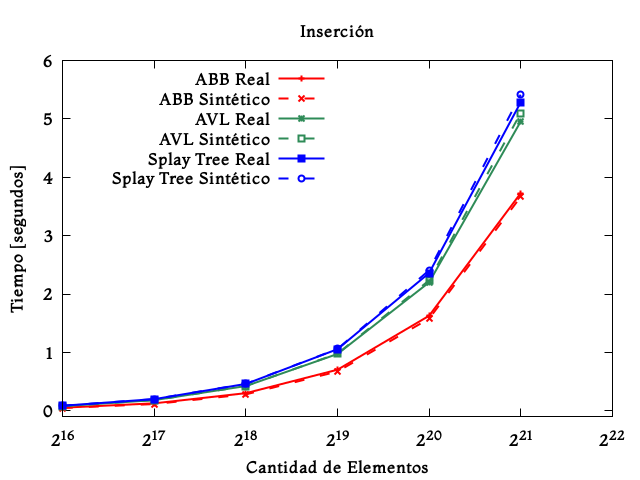
\includegraphics[scale=0.65]{random_insercion.png}
\end{center}
\end{figure}

\begin{figure}[H]
\begin{center}
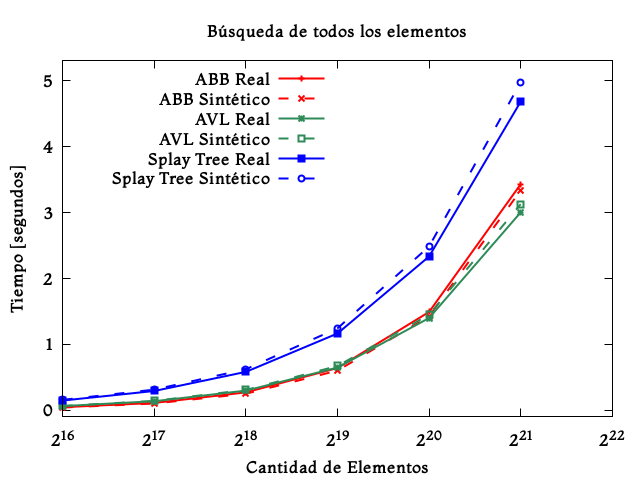
\includegraphics[scale=0.65]{random_busquedanormal.png}
\end{center}
\end{figure}

\begin{figure}[H]
\begin{center}
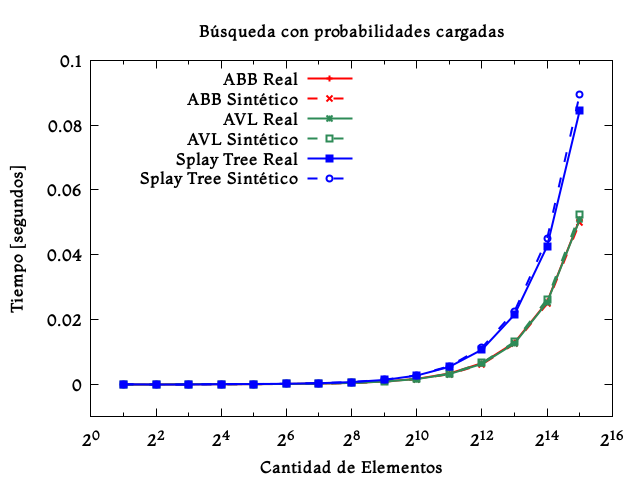
\includegraphics[scale=0.65]{random_busquedacargada.png}
\end{center}
\end{figure}

\begin{figure}[H]
\begin{center}
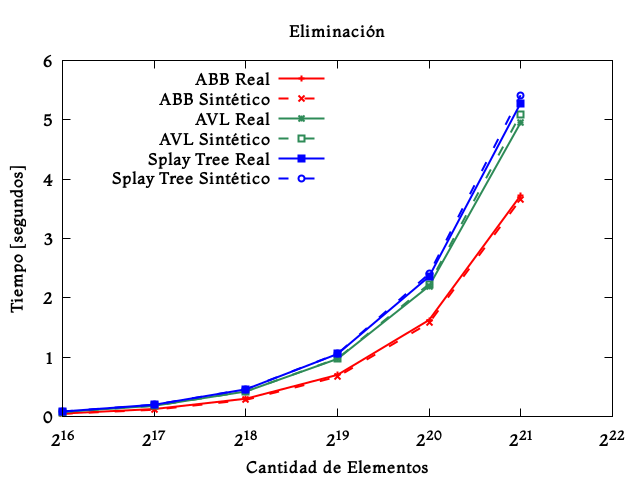
\includegraphics[scale=0.65]{random_eliminacion.png}
\end{center}
\end{figure}

Como se puede ver, las mediciones relevantes son cuando los elementos en la estructura superan los $2^{16}$, razón por la que los gráficos parten de ese valor. Antes de ello las diferencias son tan mínimas que no vale la pena analizarlas.

\subsection{Tiempos en Caso Degenerado}
\label{subsec:res_degenerado}

Aquí vale lo mismo que se acaba de decir al final de la subsección anterior, el eje $x$ (tiempo) se escala para mostrar sólo los valores a partir de los cuales la diferencia se hace significativa.

\begin{figure}[H]
\begin{center}
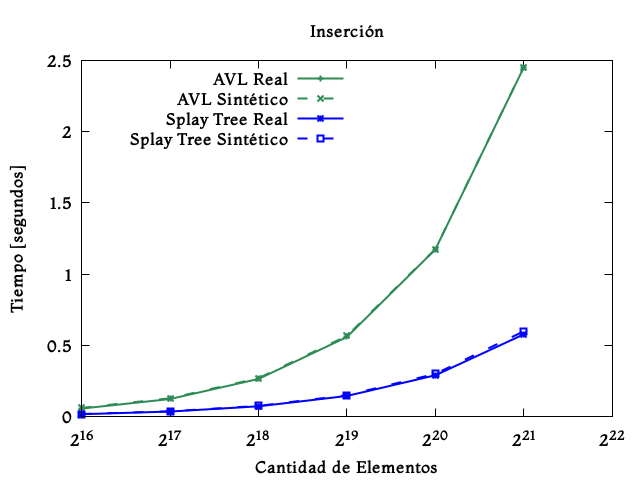
\includegraphics[scale=0.65]{degenerado_insercion.png}
\end{center}
\end{figure}

\begin{figure}[H]
\begin{center}
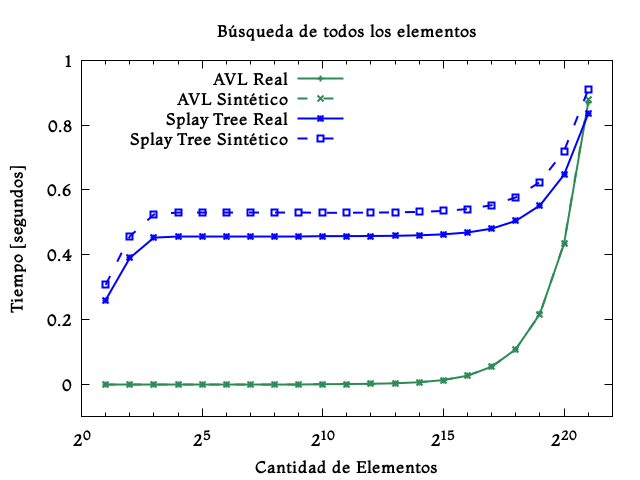
\includegraphics[scale=0.65]{degenerado_busquedanormal.png}
\end{center}
\end{figure}

\begin{figure}[H]
\begin{center}
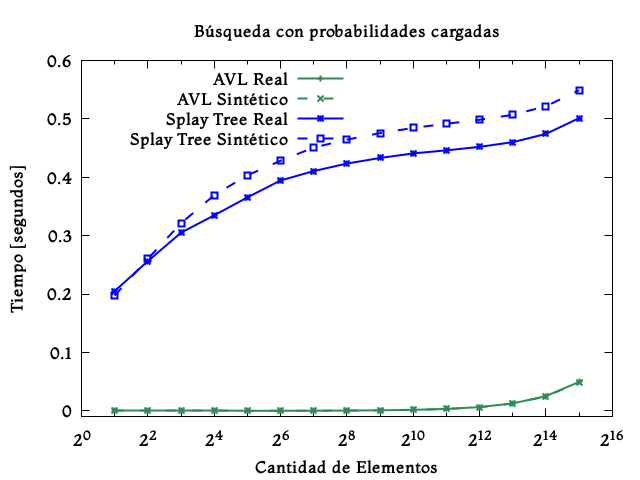
\includegraphics[scale=0.65]{degenerado_busquedacargada.png}
\end{center}
\end{figure}

\begin{figure}[H]
\begin{center}
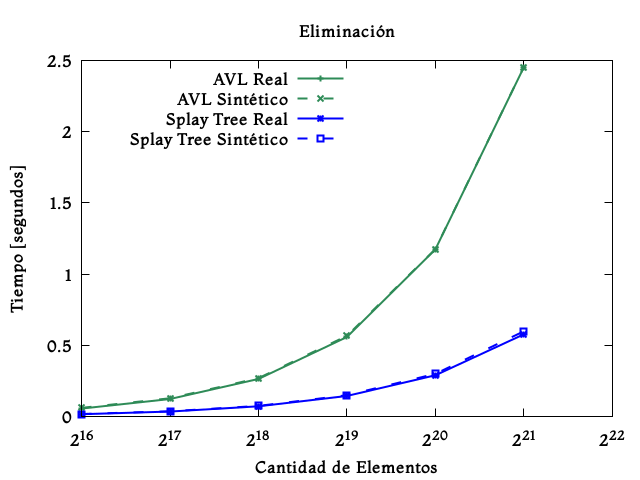
\includegraphics[scale=0.65]{degenerado_eliminacion.png}
\end{center}
\end{figure}

Vale la pena explicar por qué no se incluye la medición para el Árbol de Búsqueda Binaria en este caso.\\

Como ya se dijo en las hipótesis, los ABB en el caso degenerado (esto es, cuando las cadenas se insertan en orden lexicográfico) se convierten en listas enlazadas, asunto que puede no parecer tan importante al principio, pero en la próxima sección se discutirá por qué esto es importante.\\

Resulta, pues, que una medición verídica implica verificar que los resultados obtenidos sean de calidad, o sea, se necesita tomar un promedio sobre las mediciones y minimizar el error. Esto elimina las mediciones ``con suerte'' en las que un algoritmo puede hacerlo muy bien o muy mal. Entonces, lo que pasó con las mediciones para un ABB al principio fue la obtención de un fenómeno bastante conocido llamado \textbf{Segmentation Fault}.\\

Pues bien, la estructura está bien hecha y pasa todos los tests de memoria, por lo que un \emph{segfault} da para pensar. Corriéndolo con \texttt{valgrind}, la herramienta arrojó que el programa había incurrido en un \textbf{Stack Overflow}.\\

Para solucionar un Stack Overflow (o sea, demasiada memoria en el Stack), se puede usar la función \texttt{setrlimit} definida en el header \texttt{sys/resource.h} y aumentar el tamaño máximo del stack para un proceso.\\

El resultado fue lo que sigue (ignore el hecho de que el directorio de trabajo tiene que ver con otro ramo):

\begin{figure}[H]
\begin{center}
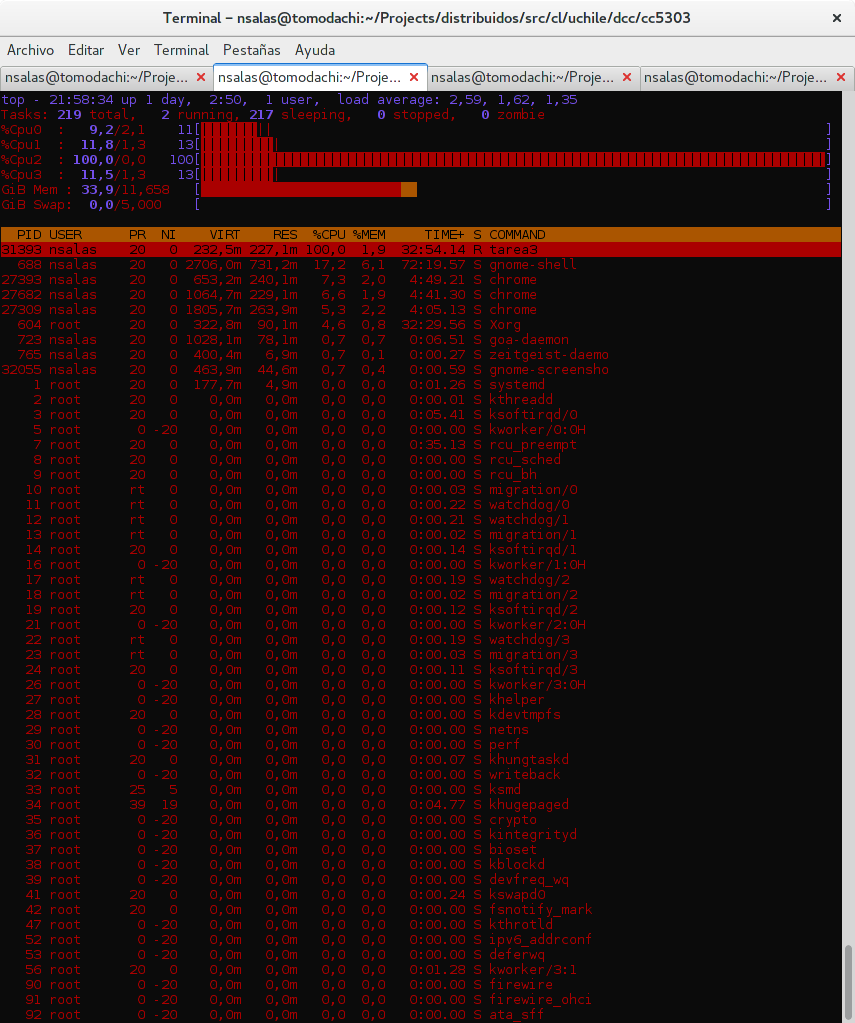
\includegraphics[scale=0.4]{tiempo_abb_degenerado.png}
\end{center}
\end{figure}

Como muestra el comando \texttt{top}, el proceso llevaba 32 minutos sin poder terminar siquiera una iteración. Para una medición certera se debe iterar por lo menos diez veces antes de concluir que no hay error. Asumiendo que el programa terminaba a los 40 minutos (siendo generoso), diez iteraciones hubiesen tomado 400 minutos, que corresponden a 6 horas y 40 minutos.\\

Este resultado ciertamente que será discutido en la interpretación.

\newpage
\section{Análisis e Interpretación de los Datos}



\newpage
\section{Apéndices}
\subsection{Dominio Básico}
\label{subsec:apen_dombasico}
Como se mencionaba al principio, en este apéndice se introducen algunos conceptos necesarios para entender este informe. Dichos conceptos son recursión, punteros y estructuras de datos. Aquí se da una definición lo suficientemente sucinta para entender el informe, sin embargo, también se proveen links para entender estos conceptos a fondo, en caso de que el lector tenga interés en ello.

\subsubsection{Recursión}

Recursión, en general, es un concepto que indica que alguna cosa depende de sí misma. En el área de ciencias de la computación, la recursión de una función indica que calcular el valor de ella depende de una invocación a ella misma, generalmente con un argumento distinto. Por ejemplo, dado que las potencias son recursivas, se puede calcular la $n$-ésima potencia de 2 como sigue:

\begin{verbatim}
int potencia_de_2(int n){
  if(n==0) return 1;
  return potencia_de_2(n-1);
}
\end{verbatim}

Como se aprecia, esta función se calcula invocándose a sí misma con un argumento distinto. La segunda línea indica que cuando $n$ vale 0, entonces se retorna 1 y entonces la \emph{recursión se detiene}. Entender este concepto es fundamental para entender estructuras de datos recursivas. Esto se explica más adelante.\\

Existen muchos otros puntos de vista asociados a la reccursión. Para ir más allá del alcance de este informe se puede revisar la entrada de Wikipedia: https://es.wikipedia.org/wiki/Recursi\%C3\%B3n.

\subsubsection{Punteros}
Un puntero es una variable que almacena una dirección en memoria. Aunque la definición es correcta y no parece que haya mucho más que decir, es necesario entender algunas cosas.\\

Los punteros tienen tipos, es decir, un puntero puede apuntar hacia una dirección de memoria que almacena \texttt{int}, o \texttt{char}, o \texttt{struct arbol}. Al acceder a las direcciones de memoria a la que los punteros apuntan, lo único que se hace es \textbf{interpretar el pedazo de memoria indicado como el tipo del puntero}. O sea, si en una aplicación existe un puntero a \texttt{int} y se accede a él. Se toman 4 bytes de memoria (tamaño de un \texttt{int}) y se interpretan como si fuera un entero. Lo mismo sucede con las estructuras de datos (se explican en la próxima subsección).\\

Para este trabajo, los punteros son importantes porque permiten \emph{desacoplar} el espacio en el que habita una estructura de datos grandes, es decir, no es necesario que los datos residan en bloques continuos de memoria, gracias a los punteros, se puede acceder a estos datos sin tener que duplicar las entradas de cada nodo en los árboles.\\

Los punteros son un área compleja y muy interesante de los lenguajes de programación. El profesor Jerry Cain en Stanford explica el concepto bastante bien en las clases del curso CS107 - Programming Paradigms, que se puede ver en YouTube: https://www.youtube.com/watch?v=jTSvthW34GU\&list=PL9D558D49CA734A02.

\subsubsection{Estructura de Datos}
Una estructura de datos es un conjunto de datos que se agrupan en otro. Puede parecer no muy potente al principio, pero añadiendo el concepto de recursión y punteros es posible potenciarlas bastante, y es precisamente esta funcionalidad del lenguaje \texttt{C} la que permite escribir árboles tan fácilmente. Supóngase que se necesita crear una estructura árbol que almacene números, entonces lo único que hay que hacer es lo siguiente:
\begin{verbatim}
struct arbol{
  int valor;
  struct arbol *hijo_derecho;
  struct arbol *hijo_izquierdo;
};
\end{verbatim}
Lo que indica esta estrctura es que cada árbol tiene un valor y dos subárboles hijos: uno izquierdo y uno derecho. Cada subárbol es a su vez otro árbol que tiene la misma propiedad. Usando de los punteros, que cuando uno de ellos es \texttt{NULL}, se puede terminar la recursión. Este enfoque es el que se usa en la práctica de las implementaciones de los árboles que se usaron para este experimento.\\

Para investigar más sobre estructuras de datos se puede leer la entrada en Wikipedia. Explicar las estructuras de datos más comunes es usualmente un curso entero. https://en.wikipedia.org/wiki/Data\_structure.

\subsection{Ambiente de Ejecución}
\label{subsec:ambiente}

Entendiendo que los resultados varían dependiendo del procesador de la máquina donde se ejecuta el experimento, se incluyen las características del computador donde fue ejecutado el experimento.

\begin{center}

\begin{tabular}{ll}
  Sistema Operativo & Arch Linux, Kernel 4.2.5-1-ARCH\\
  Procesador & Intel Core i5-2500k @ 3.3 GHz\\
  Memoria Disponible & 12 GiB\\
  Tamaño de un puntero & 8 bytes (64 bits)\\
  Compilador & GCC (GNU C Compiler) 5.2.0\\
  Librería \texttt{C} & \texttt{glibc} (GNU C Library) 2.22 stable.
\end{tabular}
\end{center}

Usalmente al tamaño de un puntero (en la jerga de arquiterctura se le conoce como tamaño de palabra, o \emph{word size}) se le denomina tipo del sistema. Los más comunes son 64 bits en las máquinas nuevas y 32 bits en las máquinas un poco más viejas.

\subsection{Estadística de los resultados}
\label{subsec:estadistica}

Entendiendo que siempre existe algo que genera \emph{ruido} en las mediciones de los tiempos, es necesario \emph{normalizar} estos resultados para presentar resultados creíbles de calidad. Entre los factores que generan ruido (de los que no se pueden controlar) están:

\begin{itemize}
\item El Scheduler del Sistema Operativo
\item La aleatorización de algunos inputs
\item Uso de memoria externa en caso de necesitarla (por parte del Sistema Operativo)
\end{itemize}

Entonces, para normalizar estos datos se hace uso de la estadística. El objetivo es entregar el promedio de muchas mediciones, tal que el error asociado al promedio entregado no supere el 95\%. En adelante se dirá que un resultado es tal \emph{con un 95\% de confianza}. Para hacer esto se calculan los estimadores insesgados del promedio y la desviación estándar para los valores que se quiere calcular (en este caso, tiempo y espacio). Se repiten los experimentos hasta que el promedio ($\mu$) y la desviación estándar ($\sigma$) no superen el error esperado. Esto es, el 5\%. Matemáticamente se puede expresar de la siguiente forma.

\begin{align}
  \mu &= \sum_{i=1}^n X_i \nonumber \\
  \sigma &= \sqrt{\dfrac{\sum_{i=1}^n (X_i - \mu)^{2}}{n-1}} \nonumber \\
  \sigma &= \sqrt{\dfrac{\sum_{i=1}^n X_i^2 - n\mu^2}{n-1}} \nonumber \\
  \varepsilon &= \dfrac{\sigma}{\sqrt{n}} \nonumber
\end{align}

Con las ecuaciones anteriores se pueden calcular estimadores para el promedio ($\mu$), la desviación estandar ($\sigma$) y el error ($\varepsilon$). Para todos los experimentos se ha definido la máxima tolerancia para el error como el 5\% del promedio. Esto es:
$$\varepsilon < 0.05\cdot \mu$$
La condición anterior asegura que los datos entregados corresponden a valores estadísticamente aceptables, y eliminan casos de \emph{outliers}\footnote{Un outlier corresponde a un valor extremadamente alejado de la media, de manera que \emph{contamina} la medición del promedio.}, o casos extremadamente extraños en caso de existir inputs probabilísticos (que los hay).

\subsection{Fuente de las secuencias de ADN y ``Disclaimer''}
\label{subsec:fuente_textos}

Para la generación de secuencias de ADN se ha usado los archivos provistos por la organización \texttt{Pizza \& Chili Corpus}\footnote{http://pizzachili.dcc.uchile.cl/index.html}, quienes se dedican a la compresión de texto. Tal como se señala en el sitio web, la intención de este informe es ser un texto educacional, que muestre las diferencias entre cada estructura. El objetivo no es, en ningún caso, hacer usufructo del material para profitar de él.\\

Para obtener el texto de donde se han obtenido las secuencias de ADN se puede entrar a la página del organismo y hay que seguir los siguientes pasos:
\begin{enumerate}
\item Ir a la sección \texttt{Text Collection}.
\item Hacer clic en \texttt{DNA (gene DNA sequences)}.
\item Descargar el archivo \texttt{dna.200MB.gz}.
\end{enumerate}

Se entiende, luego de la descripción, por qué no se ha incluido este archivo junto con los fuentes, pues está disponible online y además pesa demasiado como para incluirlo en un entregable.

\subsection{Rotaciones en Árboles Binarios}
\label{subsec:rotaciones}

Explicar rotaciones.

\subsection{Explicitación de \emph{splay}}.
\label{subsec:splay_anexos}

A continuación se expone tal cual está implementada la función \emph{splay} para un Splay Tree. Está comentada, de manera que el seguimiento de lo que hace esta función es bastante simple.\\

\begin{verbatim}
static struct splay_nodo *_splay(struct splay_nodo *nodo, const char *key){
  if(nodo == NULL) return NULL;

  int cmp = strcmp(key, nodo->e->key);

  // está en la raíz. (de este subárbol al menos)
  // no hacemos zig, ni zag ni zigzag ni NADAAAAAAAAAAAAAAAAa
  if(cmp == 0) return nodo;

  if(cmp < 0){
    // sabemos que está en el lado izquierdo
    // no hay elementos a la izquierda? Termino el splay.
    if(nodo->izq == NULL) return nodo;

    int cmp2 = strcmp(key, nodo->izq->e->key);
    // Veo por donde me voy
    if (cmp2 < 0) {
      // El nodo está por la izquierda (del subárbol izquierdo).
      // Dejo el elemento en el hijo izquierdo de mi subárbol izquierdo
      nodo->izq->izq = _splay(nodo->izq->izq, key);

      // Lo quiero dejar en la raíz de mi subárbol izquierdo.
      // Me hago zig sobre mí mismo y el elem queda en la raíz del subárbol izq.
      nodo = _zig(nodo);
    } else if (cmp2 > 0) {
      // Si está por la derecha.. (del subárbol izquierdo)
      // Se trae a la raíz del hijo derecho del subárbol izquierdo de nodo el elemento
      // Cuando nodo->izq->der contiene al elemento (si existe) le hacemos zag para dejarlo
      // en la raíz subárbol izquierdo.
      nodo->izq->der = _splay(nodo->izq->der, key);
      if (nodo->izq->der != NULL)
        nodo->izq = _zag(nodo->izq);
    }

    // ya tengo el elemento en la raíz de mi subárbol izquierdo si existe.
    // si existe, un zig me lo deja en la raíz.
    if (nodo->izq == NULL) return nodo;
    return _zig(nodo);
  }

  // cmp > 0
  if(nodo->der == NULL) return nodo;
  
  int cmp3 = strcmp(key, nodo->der->e->key);
  if(cmp3 > 0){
    // está por la derecha del subárbol derecho
    // primero dejo el elemento en la raíz del hijo derecho de mi subárbol derecho
    nodo->der->der = _splay(nodo->der->der, key);

    // cuando ya está ahí, hago zag sobre mí mismo y lo dejo en la raíz de mi subárbol derecho.
    nodo = _zag(nodo);
  } else if (cmp3 < 0) {
    // Está por la izquierda de mi subárbol derecho.
    // Lo llevo a la raíz del hijo izquierdo de mi subárbol derecho primero
    nodo->der->izq = _splay(nodo->der->izq, key);

    // Lo quiero dejar en la raíz de mi subárbol derecho. Zig sobre nodo->der
    if(nodo->der->izq != NULL)
      nodo->der = _zig(nodo->der);
  }

  // Lo tengo listo. Si existe, está en nodo->der
  // y un zag sobre mí mismo lo deja en la raíz.
  if(nodo->der == NULL) return nodo;
  return _zag(nodo);
}
\end{verbatim}

\subsection{Cómo reobtener los gráficos}
\label{subsec:gnuplot}
Junto con este informe se ha entregado los sources que permiten compilar y correr el programa, pero si no se tiene acceso a ello, a partir del 17 de Diciembre de 2016 a las 0:00 horas estará disponible el código fuente en https://github.com/anachronic/tarea3-algoritmos, desde donde se podrá clonar el repositorio y los sources vía git, o bien descargarlos en formato \texttt{zip}.\\

Dentro de la carpeta \texttt{graficos/} existe un archivo llamado \texttt{graficar.gp}, que contiene el script para generar todas las imagenes usando \texttt{gnuplot}. Sin embargo, y teniendo en cuenta que los resultados son independientes de la plataforma en la que se grafique, el binario entrega todos los resultados en archivos terminados en \texttt{.dat}, en que los nombres de los archivos indican a qué experimento corresponde. Con esos archivos se puede graficar en cualquier otro programa, con Excel, MATLAB, usando R, o la herramienta de preferencia de la persona interesada en reproducir los experimentos.\\

No obstante, se recomienda usar \texttt{gnuplot}\footnote{http://www.gnuplot.info/}.




\end{document} 
